%Einleitungstext zum Modul
Die GUI stellt dem Benutzer eine grafische Oberfläche bereit, über die er die Anwendung bedienen kann. Dazu werden dem Nutzer verschiedene Einstellungsoptionen und Möglichkeiten zur Kontrolle der Ausführung angeboten. Des Weiteren stellt dieses Modul die Ergebnisse visuell dar.
\section{Klassen}
\graphicspath{{./img/gui/}}
%Bild der Klasse aus dem Klassendiagramm (nur die Klasse jeweils)
%Dokumentation zur Klasse, öffentlichen Methoden und Konstruktor sowie:
%Signal und Slots als Methoden mit Rückgabewert Sigal bzw Slot (zur kenntlichkeit) 
Nachfolgend werden alle Klassen des Moduls aufgelistet und beschrieben.
\subsection{CMainWindow}
\includegraphics[scale=0.8,trim=115 245 460 60, clip]{CMainWindow}\\
Diese Klasse ist das Hauptfenster und beinhaltet verschiedene Widgets.
\beginSlots
\item \textbf{onSaveWorkflow} \\Speichert die Workflowkonfiguration. \\Übergabeparameter: checked: bool
\item \textbf{onSaveWorkflowAs} \\Öffnet einen Dateiauswahldialog und speichert die Workflowkonfiguration. \\Übergabeparameter: checked: bool
\item \textbf{onLoadImages} \\Öffnet einen Ordnerauswahldialog und lädt die Eingabebilder. \\Übergabeparameter: checked: bool
\item \textbf{onAdvancedLoadFiles} \\Öffnet einen Ordnerauswahldialog und lädt alte Ergebnisdaten. \\Übergabeparameter: checked: bool
\item \textbf{onWorkflowSelected} \\Wählt einen Workflow aus. \\Übergabeparameter: checked: bool
\item \textbf{onSettings} \\Öffnet einen Einstellungsdialog. \\Übergabeparameter: checked: bool
\item \textbf{onAbout} \\Öffnet einen „Über“-Dialog. \\Übergabeparameter: checked: bool
\closeMembers

\subsection{CAlgorithmSettingsView}
\includegraphics[scale=0.8,trim=132 261 355 78, clip]{CAlgorithmSettingsView}\\
Zeigt die Einstellungen für die Algorithmen in einem Baum an.
\beginMembers
\item \textbf{CAlgorithmSettingsView} (Konstruktor) \\ Speichert übergebene Parameter. \\Übergabeparameter: workflow: AWorkflow\&
\newMember{setWorkflow}{workflow: AWorkflow\&}{void}{Setzt den Workflow.}
\closeMembers
\newpage
\beginSlots
\item \textbf{onAlgorithmChanged} \\Setzt die Einstellungen des Algorithmus in Schritt \textit{step} zurück. \\Übergabeparameter: step: int
\closeMembers

\subsection{CAlgorithmSettingsSaveLoadWidget}
\includegraphics[scale=0.8,trim=70 353 280 70, clip]{CAlgorithmSettingsSaveLoadWidget}\\
Widget mit zwei Buttons zum Speichern und Laden von Einstellungen eines Algorithmus.
\beginMembers
\item \textbf{CAlgorithmSettingsSaveLoadWidget} (Konstruktor) \\ Speichert übergebene Parameter. \\Übergabeparameter: row: int, model: CAlgorithmSettingsModel\&
\closeMembers

\subsection{CSettingsDialog}
\includegraphics[scale=0.8,trim=90 330 422 71, clip]{CSettingsDialog}\\
Dialog, um globale Einstellungen zu ändern.
\beginSlots
\item \textbf{accept} \\Setzt die Einstellungen in CGlobalSettingsController.
\item \textbf{onResultDirectoryButtonClicked} \\Öffnet einen Ordnerauswahldialog, um das Ausgabeverzeichnis festzulegen. \\Übergabeparameter: checked: bool
\closeMembers

\subsection{CAlgorithmSelector}
\includegraphics[scale=0.8,trim=140 295 426 94, clip]{CAlgorithmSelector}\\
Widget, um die einzelnen Algorithmen für die Workflowschritte auszuwählen.
\beginMembers
\item \textbf{CAlgorithmSelector} (Konstruktor) \\Speichert übergebene Parameter. \\Übergabeparameter: workflow: AWorkflow\&
\newMember{setWorkflow}{workflow: AWorkflow\&}{void}{Setzt den Workflow.}
\closeMembers
\beginSignals
\item \textbf{algorithmChanged} \\ Benachrichtigt andere Klassen, dass der Algorithmus in Schritt \textit{step} geändert wurde. \\Übergabeparameter: step: int
\closeMembers

\subsection{CDataViewTabContainer}
\includegraphics[scale=0.8,trim=114 272 323 77, clip]{CDataViewTabContainer}\\
Container für verschiedene Ergebnisansichten. Die einzelnen Ansichten werden per Tabs ausgewählt.
\beginMembers
\item \textbf{CDataViewTabContainer} (Konstruktor) \\Speichert übergebene Parameter. \\Übergabeparameter: imagePreview: CImagePreviewWidget*
\closeMembers
\beginSlots
\item \textbf{onCurrentChanged} \\Legt den aktuellen Tab fest. \\Übergabeparameter: index: int
\closeMembers

\subsection{IGuiDataView}
\includegraphics[scale=0.8,trim=147 391 594 142, clip]{IGuiDataView}\\
Bietet dem Container für die Ergebnisdarstellungen eine einheitliche Schnittstelle, um auf diese zuzugreifen.
\beginMembers
\newMemberAbstract{activate}{}{void}{Aktiviert die View. Sollte aufgerufen werden, wenn die View sichtbar wird.}
\closeMembers

\subsection{CImageView}
\includegraphics[scale=0.8,trim=60 123 225 94, clip]{CImageView}\\
Widget, das mehrere Bilder mit Markierungen darstellt.
\beginMembers
\newMember{paintEvent}{event: QPaintEvent*}{void}{Zeichnet die Bilder und Markierungen.}
\newMember{wheelEvent}{event: QWheelEvent*}{void}{Wertet event aus und zoomt die Ansicht entsprechend rein oder raus.}
\newMember{mouseMoveEvent}{event: QMouseEvent*}{void}{Verschiebt die Ansicht, wenn entsprechende Maustaste gedrückt.}
\newMember{mousePressEvent}{event: QMouseEvent*}{void}{Überprüft gedrückte Maustasten und initialisiert Startwert für nachfolgende Mausverschiebungen.}
\newMember{mouseReleaseEvent}{event: QMouseEvent*}{void}{Überprüft losgelassene Maustasten.}
\newMember{showImages}{images:vector<tuple<uint32\_t,QImage\&> >}{void}{Setzt die anzuzeigenden Bilder.}
\newMember{addConnectedMarkers}{positions:vector<tuple<uint32\_t,QVector2D> > (Liste von Tupeln aus Image-ID und 2D-Koordinate)}{void}{Zeichnet Markierungen auf dem per Image-ID angegeben Bild an der Koordinate und verbindet alle Markierungen mit Linien.}
\closeMembers

\subsection{CInputImageView}
\includegraphics[width=\linewidth,trim=73 237 23 72, clip]{CInputImageView}\\
Zeigt die ausgewählten Eingabebilder unverändert an.
\beginMembers
\newMember{applyData}{packet:*CImageDataPacket}{void}{Setzt die Bilder, um ausgewählte davon anzeigen zu können. Siehe: onImagesSelected}
\newMember{activate}{}{void}{Emittiert relevantImagesChanged.}
\closeMembers
\beginSlots
\item \textbf{onImagesSelected} \\Zeigt die in images angegeben Bilder an. \\Übergabeparameter: images:vector<uint32\_t>\&
\closeMembers
\beginSignals
\item \textbf{relevantImagesChanged} \\ Sendet alle verfügbaren Bilder als aktuell relevante Bilder. \\Übergabeparameter: images:vector<uint32\_t>\&
\closeMembers

\subsection{CDepthMapView}
\includegraphics[width=\linewidth,trim=73 242 23 73, clip]{CDepthMapView}\\
Zeigt die ausgewählten Tiefenkarten an.
\beginMembers
\newMember{applyData}{packet:*CDepthMapDataPacket}{void}{Setzt die Tiefenkarten, um ausgewählte davon anzeigen zu können. Siehe: onImagesSelected}
\newMember{activate}{}{void}{Emittiert relevantImagesChanged.}
\closeMembers
\beginSlots
\item \textbf{onImagesSelected} \\Zeigt die Tiefenkarten zu den in images angegeben Bilder an. \\Übergabeparameter: images:vector<uint32\_t>\&
\closeMembers
\beginSignals
\item \textbf{relevantImagesChanged} \\ Sendet alle verfügbaren Bilder, zu denen eine Tiefenkarte existiert, als aktuell relevante Bilder. \\Übergabeparameter: images:vector<uint32\_t>\&
\closeMembers

\subsection{CFeatureView}
\includegraphics[width=\linewidth,trim=73 228 23 73, clip]{CFeatureView}\\
Zeigt die ausgewählten Bilder mit Features und Matches an.
\beginMembers
\newMember{applyData}{packet:*CImageDataPacket}{void}{Setzt die Bilder, um ausgewählte davon anzeigen zu können. Siehe: onImagesSelected}
\newMember{applyData}{packet:*CFeatureDataPacket}{void}{Setzt die Features, die auf den Bildern angezeigt werden sollen.}
\newMember{activate}{}{void}{Emittiert relevantImagesChanged.}
\closeMembers
\beginSlots
\item \textbf{onImagesSelected} \\Zeigt die in images angegeben Bilder an. \\Übergabeparameter: images:vector<uint32\_t>\&
\closeMembers
\beginSignals
\item \textbf{relevantImagesChanged} \\ Sendet alle verfügbaren Bilder, zu denen es Features gibt, als aktuell relevante Bilder. \\Übergabeparameter: images:vector<uint32\_t>\&
\closeMembers

\subsection{C3dView}
\includegraphics[width=\linewidth,trim=116 169 97 110, clip]{C3dView}\\
Widget zur Darstellung von 3D-Daten wie Point-Clouds, Meshes und Posen.
\beginMembers
\item \textbf{C3dView} (Konstruktor) \\ Speichert übergebene Parameter. \\Übergabeparameter: modelTypeComboBox: QComboBox\&
\newMember{activate}{}{void}{Leere Implementierung.}
\newMember{applyData}{packet:*CPclDataPacket}{void}{Setzt die anzuzeigende Point-Cloud.}
\newMember{applyData}{packet:*CPoseDataPacket}{void}{Setzt die anzuzeigenden Posen.}
\closeMembers
\beginSlots
\item \textbf{onCurrentIndexChangedModelType} \\Zeigt den per index definierten Modelltyp an. \\Übergabeparameter: index: int
\closeMembers
\subsection{E3dModelType}
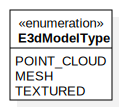
\includegraphics[scale=0.8,trim=85 428 648 70, clip]{E3dModelType}\\
Definiert die möglichen Darstellungen des Modells.

\subsection{CImagePreviewWidget}
\includegraphics[scale=0.8,trim=156 178 300 110, clip]{CImagePreviewWidget}\\
Widget zur Vorschau der Eingabebilder.
\beginMembers
\item \textbf{CImagePreviewWidget} (Konstruktor) \\Zeigt eine Vorschau der angegeben Bilder an. \\Übergabeparameter: images: vector<tuple<uint32\_t,QIcon\&> >
\newMember{setImages}{images: vector<tuple<uint32\_t,QIcon\&> >}{void}{Zeigt eine Vorschau der angegebenen Bilder an.}
\closeMembers
\beginSlots
\item \textbf{onRelevantImagesChanged} \\Filtert die angezeigten Bilder, so dass nur noch die in images angegebenen Bilder angezeigt werden. \\Übergabeparameter: images: vector<uint32\_t>\&
\closeMembers
\beginSignals
\item \textbf{imagesSelected} \\Sendet alle ausgewählten Bilder. \\Übergabeparameter: images:vector<uint32\_t>\&
\closeMembers

\subsection{CImagePreviewItem}
\includegraphics[scale=0.8,trim=125 228 297 78, clip]{CImagePreviewItem}\\
Ein Item, das eine Image-ID speichert, und nur zusammen mit CImagePreviewWidget verwendet werden sollte.
\beginMembers
\item \textbf{CImagePreviewItem} \\Speichert die übergebenen Parameter. \\Übergabeparameter:  icon: QIcon\&, text: QString\&, imageId: uint32\_t)
\newMember{getImageId}{}{uint32\_t}{Gibt die Image-ID des Bildes zurück.}
\closeMembers

\subsection{CLogWidget}
\includegraphics[scale=0.8,trim=132 227 260 86, clip]{CLogWidget}\\
Dieses Widget stellt das Log in der Benutzeroberfläche dar.
\beginSlots
\item \textbf{onNewLogMessage} \\Fügt die Nachricht an das Log an. \\Übergabeparameter: message: QString, time: QString, type: QString
\item \textbf{onStateChangedDebug} \\Legt fest, ob Debug Meldungen angezeigt werden. \\Übergabeparameter: state: int
\item \textbf{onStateChangedInfo} \\Legt fest, ob Info Meldungen angezeigt werden. \\Übergabeparameter: state: int
\item \textbf{onStateChangedWarning} \\Legt fest, ob Warning Meldungen angezeigt werden. \\Übergabeparameter: state: int
\item \textbf{onStateChangedError} \\Legt fest, ob Error Meldungen angezeigt werden. \\Übergabeparameter: state: int
\closeMembers

\subsection{CDatasetSelector}
\includegraphics[scale=0.8,trim=236 260 387 110, clip]{CDatasetSelector}\\
Diese Klasse dient der Umsetzung des Kann-Kriteriums zur Unterstützung der Ausführung mehrerer Datensätze mit dem gleichen Workflow. Der Entwurf der Klasse wird, falls das Kriterium umgesetzt wird, während der Implementierung ausgearbeitet.

\section{Pakete}

\subsection{AlgorithmSettings}
%Bild des Pakets mit vereinfachter Klassendarstellung
\includegraphics[width=\linewidth, trim=195 195 25 121, clip]{paket_AlgorithmSettings}
%Begründung / Dokumentation / Erklärung zum Paket
Das Paket AlgorithmSettings ist für die Einstellungen der Algorithmen verantwortlich. Hauptteil der AlgorithmSettings ist die Klasse CAlgorithmSettingsView, die die Einstellungen darstellt und über die der Nutzer Änderungen machen kann. Diese arbeitet dazu mit dem Einstellungs-Modul und der Klasse CAlgorithmSettingsSaveLoadWidget zusammen. Letztere stellt Optionen zum Speichern und Laden von Einstellungen für einen Algorithmus zu Verfügung.

\subsection{GlobalSettings}
\includegraphics[width=\linewidth, trim=407 300 25 155, clip]{paket_GlobalSettings}
Das Paket GlobalSettings ist für die Benutzeroberfläche der globalen Einstellungen zuständig. CSettingsDialog stellt dafür die Benutzeroberfläche bereit und gibt Änderungen an den CGlobalSettingsController weiter.

\subsection{AlgorithmSelector}
\includegraphics[width=\linewidth, trim=388 270 27 130, clip]{paket_AlgorithmSelector}
Das Paket AlgorithmSelector bietet dem Nutzer die Auswahl verschiedener Algorithmen für die einzelnen Arbeitsschritte an. Dazu arbeitet die Klasse CAlgorithmSelector mit dem Modul Workflow zusammen.

\subsection{ImageViews}
\includegraphics[width=\linewidth, trim=270 140 20 63, clip]{paket_ImageViews}
Das Paket ImageViews enthält Ergebnisdarstellungen, die in Form eines Bilder erfolgen. Dazu zählen die Anzeige der Eingabebilder (CInputImageView), der Tiefenkarten (CDepthMapView) und der Features (CFeatureView). Die Ansichten sind alle von CImageView abgeleitet, das ein Widget für eine parallele Ansicht von mehreren Bildern ist. IGuiDataView stellt ein einheitliches Interface für alle Ergebnisanzeigen bereit. Die aktuelle Anzeige wählt der Nutzer mittels Tabs in CDataViewTabContainer aus. Wird eine Anzeige ausgewählt, wird sie darüber per activate informiert und gibt dann die aktuell relevanten Bilder dem CImagePreviewWidget bekannt.

\subsection{3dView}
\includegraphics[width=\linewidth, trim=277 212 25 210, clip]{paket_3dView}
Das Paket 3dView ist für die Darstellung von 3D-Daten verantwortlich. Dazu greift es auf die Klasse PCLVisualizer aus der Bibliothek PCL zu, die wiederum auf das QVTKWidget von VTK zurückgreift. Zur Auswahl des darzustellenden Modell-Typs wird eine QComboBox verwendet.

\subsection{ImagePreview}
\includegraphics[width=\linewidth, trim=385 180 9 320, clip]{paket_ImagePreview}
Die ImagePreview stellt eine Vorschau der Eingabebilder dar. Diese Aufgabe ist bereits maßgeblich in QListWidget enthalten. Dementsprechend erbt CImagePreviewWidget davon.

\subsection{MainWindow}
\includegraphics[width=\linewidth, trim=580 325 20 150, clip]{paket_MainWindow}
Hauptaufgabe des Pakets MainWindow ist die Verwaltung der Menüleiste. Führt der Nutzer eine Aktion im Menü aus, dann wird die entsprechende Methode in CMainWindow aufgerufen. Unter anderem wird über das Menü die Auswahl der Workflows angeboten. Dazu wird auf die Klasse CWorkflowManager aus dem Modul Workflow zurück gegriffen.

\subsection{Logger}
\includegraphics[width=\linewidth, trim=545 360 25 140, clip]{paket_Logger}
Der Logger gibt auftretende Meldungen in einer Textbox aus. CLogWidget greift zur Darstellung dazu auf QPlainTextEdit zurück. Die Nachrichten erhält die Klasse per Signal von CLogController und fügt diese dann unten an. Wird eine der ComboBoxen zur Darstellung einzelner Warnstufen geändert, wird die gesamte Ausgabe neu erzeugt und dabei die Nachrichten von CLogHistory geholt.

\section{Entwurfsmuster}
\subsection{Model-View-Controller (MVC)}
Die GUI ist die View des Entwurfsmusters MVC. Dementsprechend sind die Klassen möglichst minimal gehalten und die Verwaltung und Bearbeitung von Daten sind in andere Module ausgelagert. Dadurch wird sichergestellt, dass die GUI bei Bedarf leicht ausgetauscht werden kann und so bspw. eine Ausführung über die Konsole wie in denn Kann-Kriterien einfach umgesetzt werden kann.

\subsection{Beobachter}
Innerhalb der GUI und auch bei der Kommunikation mit anderen Modulen werden Qt-Signale verwendet. Diese implementieren das Entwurfsmuster Beobachter. Durch die Möglichkeit der einfachen Verbindung zwischen Klassen können neue Klassen hinzugefügt werden und als Beobachter fungieren, ohne dass an der beobachteten Klassen etwas geändert werden muss.
% verwendete Entwurfsmuster aufzählen erklären etc mit verinfachtem Diagramm (Klassen ohne Inhalt nur die Namen)

\section{Klassendiagramm}
% Klassendiagramm des Moduls
\includegraphics[width=\linewidth, trim=30 250 20 30, clip]{overview}

%Bitte jeweils kleine Einleitungstexte usw in Unterkapitel gerne auch in Textform Erklärungen zufügen und auf mögliche erweiterungen durch die kann Kriterien eingehen soweit nötig !